\documentclass[margin=2mm]{standalone}
\usepackage{tikz}
\usepackage{circuitikz}
\usepackage{siunitx} 
\usepackage{pst-circ}
\usetikzlibrary{calc,positioning,shapes.geometric,backgrounds,fit,shadows.blur,arrows,arrows.meta,decorations.markings}
\tikzset{
  hole/.style = {fill = #1, circle, minimum width = 2.5mm, inner sep = 0mm},
  wire/.style = {draw = #1, line width = .5mm},
  label/.style = {black!50!white, font=\sffamily, anchor = center},
  text/.style = {white, font=\sffamily, anchor = right},
  line/.style={-,blur shadow, line width = 5}
}
\begin{document}
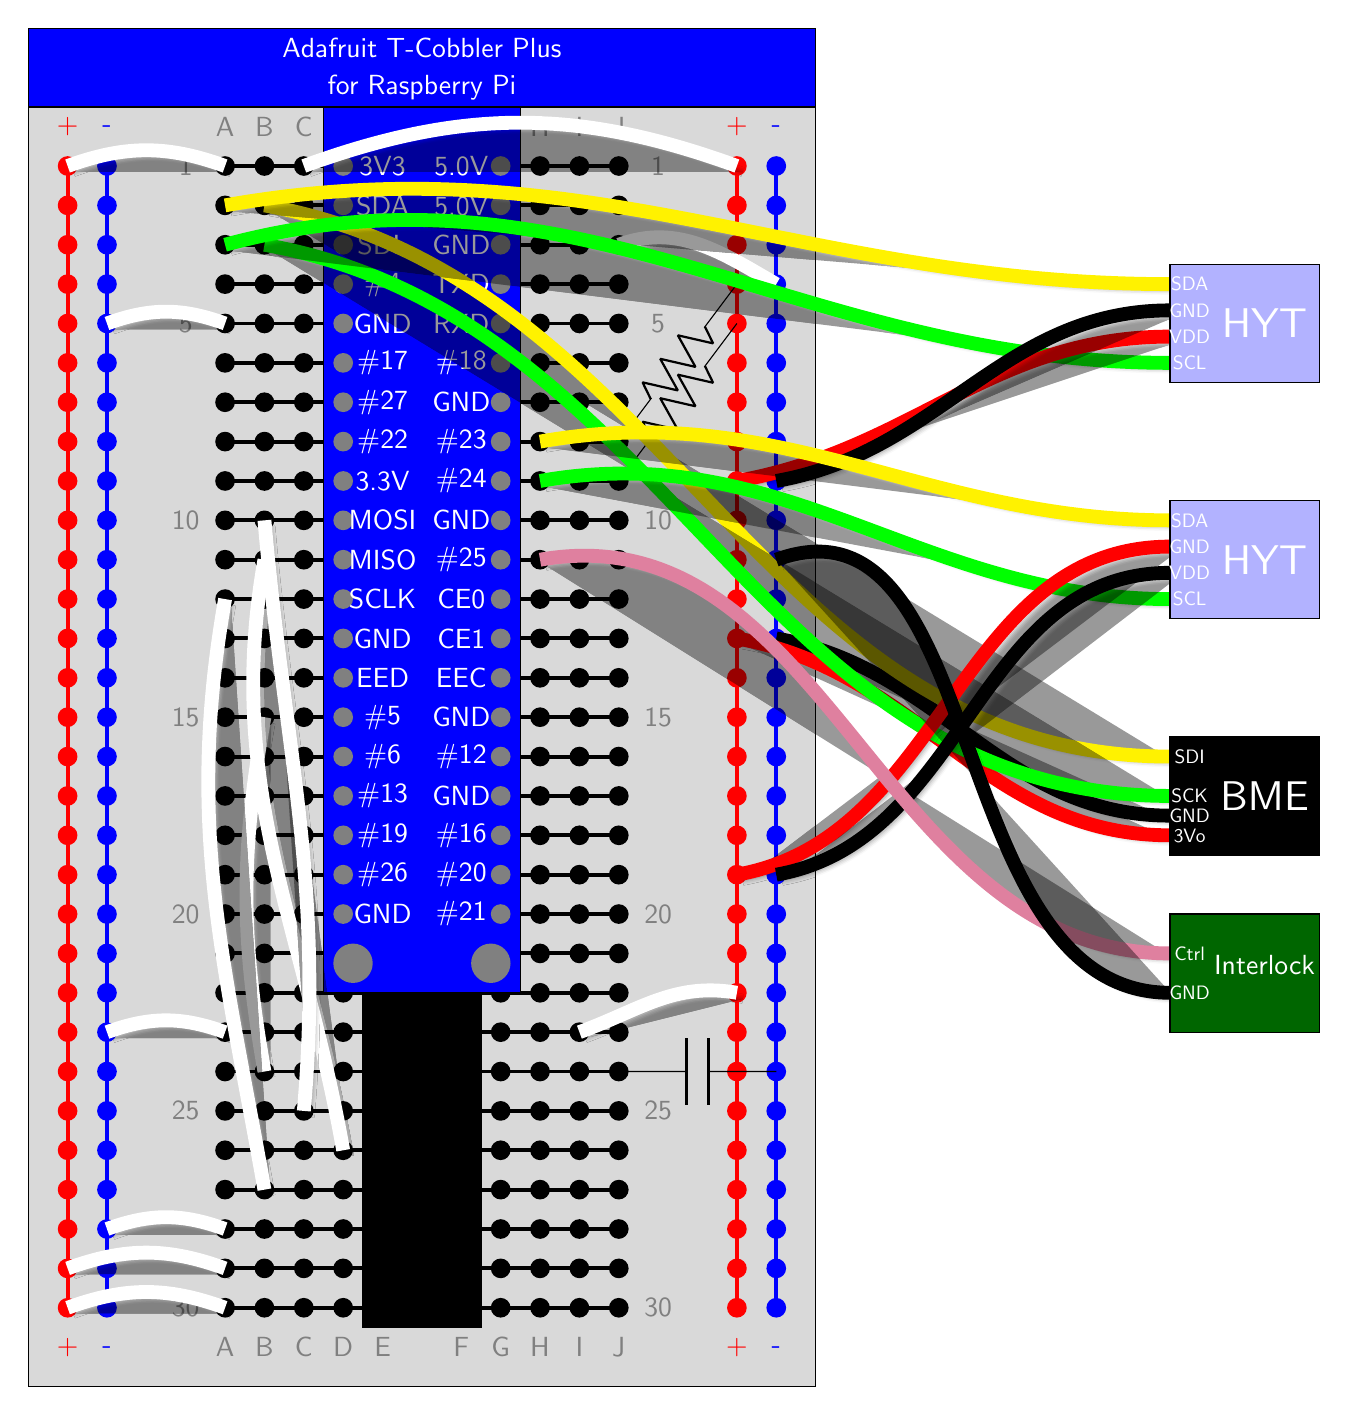
\begin{tikzpicture}[x=5mm,y=5mm]
  \draw[fill=black!15!white] (-4,-1) rectangle (16,32);
  \draw[wire=red]  (-3,1) -- (-3,30);
  \draw[wire=blue] (-2,1) -- (-2,30);
  \draw[wire=red]  (14,1) -- (14,30);
  \draw[wire=blue] (15,1) -- (15,30);
  \foreach \yi in {1,...,30}{
    \node[hole=red]  at (-3,\yi){};
    \node[hole=blue] at (-2,\yi){};
    \node[hole=red]  at (14,\yi){};
    \node[hole=blue] at (15,\yi){};
    \foreach \xs in {0,6}{
      \draw[wire=black] (\xs+1,\yi) -- (\xs+5,\yi);
      \foreach \xi in {1,2,3,4,5}{
        \node[hole=black] at (\xi+\xs,\yi){};
      }
    }
  }
  \foreach \m/\xi in {A/1,B/2,C/3,D/4,E/5,F/7,G/8,H/9,I/10,J/11}{
    \node[label=90] at (\xi,0) {\m};
    \node[label=90] at (\xi,31) {\m};
  }
  \foreach \m/\yi in {30/1,25/6,20/11,15/16,10/21,5/26,1/30}{
    \node[label=90] at (0,\yi) {\m};
    \node[label=90] at (12,\yi) {\m};
  }
  \foreach \m/\xi in {+/-3,+/14}{
    \node[red] at (\xi,0) {\m};
    \node[red] at (\xi,31) {\m};
  }
  \foreach \m/\xi in {-/-2,-/15}{
    \node[blue] at (\xi,0) {\m};
    \node[blue] at (\xi,31) {\m};
  }
  \draw[fill=blue] (-4,31.5) rectangle (16,33.5);
  \draw[fill=blue] (3.5,31.5) rectangle (8.5,9);
  \draw[fill=black] (4.5,9) rectangle (7.5,0.5);
  \foreach \yi in {11,...,30}{
    \node[hole=gray] at (4,\yi){};
    \node[hole=gray] at (8,\yi){};
  }
  \foreach \m/\yi in {3V3/30,SDA/29,SDL/28,\#4/27,GND/26,\#17/25,\#27/24,\#22/23,3.3V/22,MOSI/21,MISO/20,SCLK/19,GND/18,EED/17,\#5/16,\#6/15,\#13/14,\#19/13,\#26/12,GND/11}{ 
    \node[white, font=\sffamily, align=right] at (5,\yi) {\m};
  }
  \foreach \m/\yi in {5.0V/30,5.0V/29,GND/28,TXD/27,RXD/26,\#18/25,GND/24,\#23/23,\#24/22,GND/21,\#25/20,CE0/19,CE1/18,EEC/17,GND/16,\#12/15,GND/14,\#16/13,\#20/12,\#21/11}{ 
    \node[white, font=\sffamily, align= left] at (7,\yi) {\m};
  }
  \node[white, font=\sffamily] at (6,33) {Adafruit T-Cobbler Plus};
  \node[white, font=\sffamily] at (6,32) {for Raspberry Pi};
  \foreach \x in {4.25,7.75}{
    \node[fill = gray, circle, minimum width = 5mm, inner sep = 1mm] at (\x,9.75){};
  }
  \draw[line,white] (-3,30) to [out=20,in=160] (1,30);
  \draw[line,white] (-2,26) to [out=20,in=160] (1,26);
  \draw[line,white] (3,30) to [out=20,in=160] (14,30);
  \draw[line,white] (11,28) to [out=20,in=150] (15,27);
  \draw[line,white] (-3,1) to [out=20,in=160] (1,1);
  \draw[line,white] (-3,2) to [out=20,in=160] (1,2);
  \draw[line,white] (-2,3) to [out=20,in=160] (1,3);
  \draw[line,white] (-2,8) to [out=20,in=160] (1,8);
  \draw[line,white] (2,7) to [out=100,in=-100] (2,16);
  \draw[-,blur shadow={shadow blur steps=1},white, line width = 5] (4,5) to [out=100,in=-100] (2,20);
  \draw[line,white] (3,6) to [out=85,in=-85] (2,21);
  \draw[line,white] (2,4) to [out=100,in=-100] (1,19);
  \draw[line,white] (10,8) to [out=20,in=170] (14,9);
  \draw (11,23) to[resistor] (14,27);
  \draw (11,22) to[resistor] (14,26);
  \draw (11,7) to[capacitor] (15,7);
  % bme
  \draw[line,black] (15,18) to [out=-10,in=180] (25,13.5);
  \draw[line,red] (14,18) to [out=-10,in=180] (25,13);
  \draw[line,yellow] (2,29) to [out=-10,in=180] (25,15);
  \draw[line,green] (2,28) to [out=-10,in=180] (25,14);
  \draw[fill=black] (25,12.5) rectangle (28.8,15.5);
  \node[white,font=\sffamily,scale =1.5] at (27.4,14) {BME};
  \foreach \m/\yi in {SDI/15,GND/13.5,3Vo/13,SCK/14}{ \node[white,font=\sffamily,scale=0.7] at (25.5,\yi) {\m};
  }
  
  % hyt
  \draw[line,yellow] (1,29) to [out=10,in=180] (25,27);
  \draw[line,green] (1,28) to [out=15,in=180] (25,25);
  \draw[line,red] (14,22) to [out=10,in=180] (25,25.667);
  \draw[line,black] (15,22) to [out=10,in=180] (25,26.333);
  \draw[fill=white!70!blue] (25,27.5) rectangle (28.8,24.5);
  \node[white,font=\sffamily,scale =1.5] at (27.4,26) {HYT};
  \foreach \m/\yi in {SDA/27,GND/26.333,VDD/25.667,SCL/25}{ \node[white,font=\sffamily,scale=0.7] at (25.5,\yi) {\m};
  }

  % hyt
  \draw[line,yellow] (9,23) to [out=10,in=180] (25,21);
  \draw[line,green] (9,22) to [out=10,in=180] (25,19);
  \draw[line,red] (14,12) to [out=10,in=180] (25,20.333);
  \draw[line,black] (15,12) to [out=10,in=180] (25,19.667);
  \draw[fill=white!70!blue] (25,21.5) rectangle (28.8,18.5);
  \node[white,font=\sffamily,scale=1.5] at (27.4,20) {HYT};
  \foreach \m/\yi in {SDA/21,GND/20.333,VDD/19.667,SCL/19}{ \node[white,font=\sffamily,scale=0.7] at (25.5,\yi) {\m};
  }
  % int controll
  \draw[line,white!50!purple] (9,20) to [out=10,in=180] (25,10);
  \draw[line,black] (15,20) to [out=20,in=180] (25,9);
  \draw[fill=black!60!green] (25,11) rectangle (28.8,8);
  \node[white,font=\sffamily,scale =1] at (27.4,9.7) {Interlock};
  \foreach \m/\yi in {Ctrl/10,GND/9}{ \node[white,font=\sffamily,scale=0.7] at (25.5,\yi) {\m};
  }
  

  
\end{tikzpicture}
\end{document}